%
% 第四章
%
\chapter{基于UEFI的硬盘文件安全加载策略的详细设计}
UEFI环境中硬盘文件的安全加载依赖于UEFI固件系统中对UEFI各个启动阶段核心代码的可信验证,和对特定文件
系统协议栈驱动程序和硬盘ESP分区中文件的可信测量,本文在第三章中已经描述了此安全方案在基于原有UEFI BIOS
的基础上进行的阶段设计和可信度量模块的设计。在本章将会针对第三章中的设计方案提出对应的具体实施过程,其中
包括可信度量模块各个模块的详细设计和根据各个启动阶段的特点进行的启动阶段安全方案详细设计。

%
% 4.1节
%
\section{可信度量驱动的实现}
此安全方案设计的DXE阶段可信度量驱动程序属于DXE服务型驱动,其中包含了几个主要的功能模块,他们分别是
第三章中系统结构图提出的可信度量值计算模块、固件文件系统和硬盘文件系统访问模块、BMC通信模块、驱动程序
度量模块和硬盘文件度量模块,本节将对这些模块做更细致的介绍和实现细节。

\subsection{可信度量值计算模块}
可信度量值计算模块是对自定义SHA1散列函数的封装,用于对DXE阶段的四个UEFI文件系统协议栈驱动程序进行完整性
度量,并对BDS core进行度量;也负责在BDS阶段对硬盘文件数据进行可信测量。
\par 此度量过程采用SHA1散列值计算方法,SHA1是由NISTNSA设计为同DSA一起使用的,它对长度小于2的64次方的输入,
产生长度为160bit的散列值,因此抗穷举(brute-force)性更好。SHA-1设计时基于和MD4相同原理,并且模仿了该算法。
SHA-1是由美国标准技术局(NIST)颁布的国家标准,是一种应用最为广泛的hash函数算法,也是目前最先进的加密
技术,被政府部门和私营业主用来处理敏感的信息。而SHA-1基于MD5,MD5又基于MD4。

\begin{lstlisting}
typedef struct{
    EFI_SHA1_INIT SHA_Init;
    EFI_SHA1_UPDATE SHA_Update;
    EFI_SHA1_FINAL SHA_Final;
    EFI_SHA1_CLEAN SHA_Clean;
} EFI_SHA1_PROTOCOL;
\end{lstlisting}

代码列出的是自定义的EFI\_SHA1\_PROTOCOL协议,用于在加载DXE阶段的可信度量驱动时通过Openprotocol的启动时
服务的系统调用加载到UEFI系统的句柄数据库中。其中EFI\_SHA1\_INIT,EFI\_SHA1\_UPDATE,EFI\_SHA1\_FINAL,
EFI\_SHA1\_CLEAN为四个函数指针,用于指向位于驱动中的函数实现。SHA\_Init函数指针所指向的函数用于初始化一个
用于SHA1算法加密过程的数据结构SHA\_CTX,该结构存放弄了生成SHA1散列值的一些参数。SHA\_Update函数用于处理
大文件,将其分散成等份的较小值,并对每一块分别调用SHA\_Update生成对应的散列值。SHA\_Final函数用于将
SHA\_Update函数生成的分块的散列值通过运算形成一个最终的160bits的散列值。SHA\_Clean函数用于清除SHA\_CTX
数据结构中针对SHA1算法初始化的数据。

\begin{lstlisting}
typedef struct SHAstate_st {
    SHA_LONG h0,h1,h2,h3,h4;
    SHA_LONG Nl,Nh;
    SHA_LONG data[SHA_LBLOCK];
    unsigned int num;
} SHA_CTX;
\end{lstlisting}

在结构体SHA\_CTX中,SHA\_LONG定义为unsigned int类型,SHA-1采用160位的信息摘要,也以32位为计算长度,
就需要5个链接变量,因此h0-h4用来在SHA\_Init过程中初始化并存储这5个链接变量用于度量过程中的计算。其中
的SHA\_LBLOCK变量的扩展值为64,意味着SHA1在进行分组运算时,每一组的长度为512bits及64Bytes。

\subsection{固件文件系统访问模块}
固件文件系统访问模块用于给可信度量值计算模块提供各个阶段的核心代码和DXE阶段的文件系统协议栈驱动程序在FV
固件卷中的数据信息。需要根据FV固件卷中FFS固件文件系统的数据格式提取出对应的核心或驱动文件的Image信息
\cite{english2}。
但FV固件卷中存储的FFS格式的文件中并不只包含着可运行的EFI类型二进制文件,还有着许多标识着文件类型、文件
修改信息等众多段信息,若要对UEFI各个阶段核心代码和特定驱动文件进行度量,必须确定需要度量的EFI可执行文件
的data部分内容,以确保基准值的计算与UEFI启动过程中度量值的计算所计算的EFI数据内容统一。
\par 本节将详细说明FFS文件的存储格式以及此安全方案的固件文件系统访问模块如何进行的设计与实现。

\subsubsection{FFS文件存储格式}
根据第二章中所述的FV固件卷数据存储方式的介绍可知,FV固件中的文件以section的形式分段存储,每个数据段存储
特定的文件规格信息。但要在UEFI内存中精确的获取到核心和驱动程序文件的EFI数据内容,就需要更详细的FFS文件
存储格式研究。FV固件卷中文件的存储方式表示在图4-1中。

\begin{figure}[htb]
    % 调整图片与上文的垂直距离 %
    \vspace{0cm}   
    % 调整图片图片与中文标题、中文标题与英文标题距离 %
    \setlength{\abovecaptionskip}{0.3cm}
    % 引用/fig/目录中的图片文件 %
	\centering
    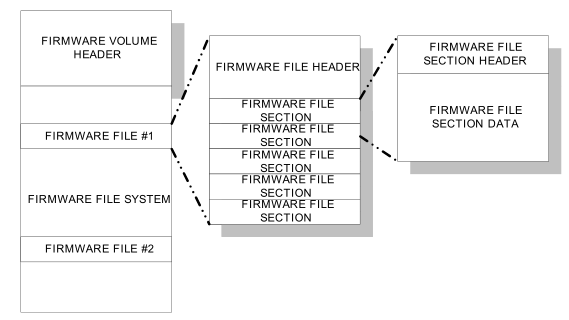
\includegraphics[width=12cm]{fv_format.png}
    % 中文标题 %
    \caption*{图 4-1 固件卷数据存储格式}
    % 调整图片英文标题与下文距离(本文标准为-0.7cm) %
    \setlength{\belowcaptionskip}{-0.7cm}
    % 英文标题 %
    \caption*{Figure 4-1 The Firmware Volume Format}
\end{figure}

如图4-1所示,符合PI规范的FV固件卷文件包含主要两部分,其中一部分是如图所示的firmware volume header
固件卷头部,另一部分是firmware volume data固件卷数据部分。其中固件卷头部用于描述此FV文件的所有属性信息,
同时也包含了一个用来标识组织固件中数据存储格式的固件文件系统的UEFI全局标识符GUID。固件卷头部不仅可以支持
UEFI特定的FFS固件文件系统,还支持一切符合PI规范的固件文件系统。
\par 当UEFI系统加载FV中的文件信息时,首先识别固件卷头部,并用名为EFI\_FIRMWARE\_VOLUME\_HEADER的
数据结构用来在UEFI内存中存储头部信息。固件卷数据部分也用GUID的形式在内存中进行唯一标识,其中UEFI规范
认可的固件文件系统GUID用EFI\_FIRMWARE\_FILE\_SYSTEM2\_GUID和EFI\_FIRMWARE\_FILE\_SYSTEM3\_GUID写死在BIOS
的固件芯片中。当单个文件内容小于16MB时,系统将采用EFI\_FIRMWARE\_FILE\_SYSTEM2\_GUID来描述固件文件
系统,若单个文件内容大于16MB,并且向后兼容SYSTEM2类型的FFS时,将采用EFI\_FIRMWARE\_FILE\_SYSTEM3\_GUID
来描述。

\begin{figure}[htb]
    % 调整图片与上文的垂直距离 %
    \vspace{0cm}   
    % 调整图片图片与中文标题、中文标题与英文标题距离 %
    \setlength{\abovecaptionskip}{0.3cm}
    % 引用/fig/目录中的图片文件 %
	\centering
    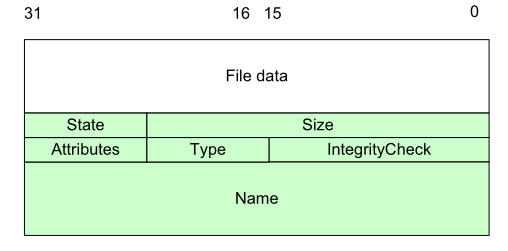
\includegraphics[width=10cm]{ffs_file_layout.png}
    % 中文标题 %
    \caption*{图 4-2 固件文件系统文件布局}
    % 调整图片英文标题与下文距离(本文标准为-0.7cm) %
    \setlength{\belowcaptionskip}{-0.7cm}
    % 英文标题 %
    \caption*{Figure 4-2 Typical FFS File Layout}
\end{figure}

\par 如图4-1所示,固件卷中每一个文件以单独的结构进行存储,文件名称为FFS file。一个文件中包含了文
件头部,用于记录文件中section内容及文件属性的信息,如图4-2中所示的文件状态、文件大小、文件名称、文件属性、
文件类型等信息,图4-2展示的是一个ffs文件的文件结构组成,其中所有的头部和数据信息都是32位对齐的。
同时包含了一组section。每一个section中也都分别包含一个section头部信息,还有section中的数据内容。
UEFI规范所规定的固件文件系统section分类及信息如表4-1。

\begin{table}[htb]
    % 设置表内行间距 %
    \renewcommand\arraystretch{1.5}
    % 设置表题目 %
	\caption*{表 4-1 固件文件系统分段信息}
	\caption*{Table 4-1 The Firmware File System Section Imformation}
    \begin{tabular*}{\hsize}{@{}@{\extracolsep{\fill}}ccl@{}}
    % 表上线和表头 %
	\toprule[0.75pt]
    名称  &数值  &\makecell[c]{描述}\\
    % 表中线和表内容 %
	\midrule[0.5pt]
	EFI\_SECTION\_COMPRESSION     &0x01  &\quad 封装了其他被压缩的分段\\
    EFI\_SECTION\_GUID\_DEFINED   &0x02  &\makecell[l]{
                                          \quad 封装部分,其中其他部分的格式由GUID\\
                                                定义\\
                                        }\\
    EFI\_SECTION\_DISPOSABLE      &0x03  &\makecell[l]{
                                          \quad 在构建过程中使用的封装部分,但执行时\\
                                                不需要\\
                                        }\\
    EFI\_SECTION\_PE32            &0x10  &\quad PE32格式信息和可执行映像\\
    EFI\_SECTION\_PIC             &0x11  &\quad 位置无关的代码段\\
    EFI\_SECTION\_DXE\_DEPEX      &0x13  &\quad DXE阶段依赖表达式\\
    EFI\_SECTION\_VERSION         &0x14  &\quad 版本号,文字和数字信息\\
    EFI\_SECTION\_RAW             &0x19  &\quad raw数据信息\\
    EFI\_SECTION\_PEI\_DEPEX      &0x1b  &\quad PEI阶段依赖表达式\\
    % 表下线 %
	\bottomrule[0.75pt]
    \end{tabular*}
    % 表格与下文距离 %
    \vspace{-0.3cm}
\end{table}

如表4-1所示,在FV固件卷中的每个section中,都对应着不同的section分类信息,其中可以看到,EFI\_SECTION\_PE32
这个section中存放着DXE驱动程序相关的关键信息,其中包含了PE32格式的说明信息,还有就是对应的EFI可执行文件,
也就是驱动程序真正的可执行代码部分内容。在此安全方案的可信度量模块中,度量的就是UEFI启动各个阶段核心代码和
驱动程序代码在FV固件卷中对应这个section里的相关信息。从表4-1中还可以看出,如EFI\_SECTION\_GUID\_DEFINED
段的信息内容可以在FV固件卷中标识驱动程序的GUID信息,这也为在UEFI启动阶段在加载驱动程序时,通过内存中的驱动
GUID和FV固件中的GUID匹配做好了实现基础。在众多section中,同样包括了如EFI\_SECTION\_VERSION这样的驱动文件
版本的文字和数字信息标识。
\par 表4-1中的EFI\_SECTION\_DXE\_DEPEX和EFI\_SECTION\_PEI\_DEPEX段的信息内容同样是两个关键的段信息,
他们分别用于表达DXE阶段和PEI阶段对应的各个驱动程序和PEIM的加载顺序,此安全方案的实现需要借助这两个驱动依赖
关系的字段来确定关键驱动加载的顺序问题,具体的依赖表达式关系及实施将在后面的小结中详细说明。

\subsubsection{固件文件访问模块详细设计}
在确定了FFS固件文件系统数据存储的具体格式之后,将在此可信度量驱动中的固件文件系统访问模块中实现UEFI内存中
的驱动文件加载方法和内存中的存储方式。此模块将调用Boot Service启动服务中的LoadImage()系统函数,在UEFI
中,所有系统服务中存储的都是具体函数的函数指针,因此真正的映像加载功能函数由CoreLoadImage()函数负责实现,
并且其他系统函数也遵循这样的命名规则。具体函数的调用过程可通过代码分析得知,为CoreLoadImage调用
CoreLoadImageCommon再最终通过CoreLoadPeImage函数进行PE32格式的文件数据加载。而这个格式也就对应上面提到
的FV中的EFI\_SECTION\_PE32段里的内容。
\par 通过CoreLoadPeImage函数来完成驱动程序在固件芯片中的加载。其中几个重要的参数包括,
Pe32Handle输入参数指定了加载到UEFI内存中
的PE32格式的映像句柄。Image参数为LOADED\_IMAGE\_PRIVATE\_DATA格式的数据结构,用于在系统内存中表示此DXE
驱动程序的详细信息,其中也包含了PE32文件格式的头部信息和data数据信息。DstBuffer参数为可选输入参数,用于
指定将此驱动文件映像存储至调用者指定的内存buffer缓存中。EntryPoint参数同样为可选参数,用于指定PE32 section
中EFI可执行文件的入口点。Attribute为32位的image属性信息参数,每一bit位分别用于表示image信息。
\par 其中IN和OUT为通过C语言\#define宏定义定义的空类型名称,用于给编码人员确定函数的输入和输出参数的设定,
UEFI实现中函数统一采用这种方式,符合UEFI规范。

\begin{lstlisting}
typedef struct {
    ......
    PE_COFF_LOADER_IMAGE_CONTEXT  ImageContext; 
    EFI_STATUS                  LoadImageStatus;
} LOADED_IMAGE_PRIVATE_DATA;
\end{lstlisting}

如上面代码所示,LOADED\_IMAGE\_PRIVATE\_DATA数据结构用于在UEFI内存中表示DXE驱动程序的完整信息,其中
Handle和EntryPoint和CoreLoadPeImage函数的参数保持一致。ImageBasePage和NumberOfPages字段用于描述此
驱动文件在内存中所占以页为单位的起始页位置和所占页数。也包括了用32位存储的驱动类型信息,其中UEFI中支持的
驱动映像类型包括:

\begin{lstlisting}
#define EFI_IMAGE_SUBSYSTEM_EFI_APPLICATION 10
#define EFI_IMAGE_SUBSYSTEM_EFI_BOOT_SERVICE_DRIVER 11
#define EFI_IMAGE_SUBSYSTEM_EFI_RUNTIME_DRIVER 12
\end{lstlisting}

他们分别表示UEFI上层应用型映像文件,启动时服务的驱动映像文件和运行时驱动映像文件,并且PE32格式的映像类型
属于EFI\_IMAGE\_SUBSYSTEM\_EFI\_RUNTIME\_DRIVER类型,可在加载驱动映像时进行类型的判别。
\par LOADED\_IMAGE\_PRIVATE\_DATA数据结构中的ImageContext关键字段为可信度量过程的主要依据,ImageContext
是一个PE\_COFF\_LOADER\_IMAGE\_CONTEXT类型结构体,用来记录驱动文件加载信息。

\begin{lstlisting}
typedef struct {
    ......
    VOID              *ImageBase;
    UINT64            ImageSize;
    ......
} PE_COFF_LOADER_IMAGE_CONTEXT;
\end{lstlisting}

其中ImageBase就是记录内存中PE32格式文件的起始地址,ImageSize提供了文件的大小,通过把PE32格式驱动映像
文件加载到指定地址,并将其记录在这两个变量中,就可以在度量时获取到驱动文件内容。

\subsection{硬盘文件系统访问模块}
硬盘文件系统访问模块提供FAT文件系统中ESP分区内系统文件数据的加载过程,此模块由BDS core代码调用,用来
将指定硬盘文件数据加载到UEFI内存中,过程如下所示。

\begin{lstlisting}
    Status = VolumeInterface->OpenVolume(VolumeInterface, &RootIo);
    Status = RootIo->Open(RootIo, &FileIo,imgdir,EFI_FILE_MODE_READ, EFI_FILE_READ_ONLY);
    Status = FileIo->Read(FileIo, &Size, (VOID *)DesAddr);
\end{lstlisting}

如代码清单所示,展示了硬盘文件访问过程中几个重要的过程,包括了硬盘卷的打开、根索引阶段的获取、文件的搜索
和文件数据的读取。

\begin{figure}[htb]
    % 调整图片与上文的垂直距离 %
    \vspace{0cm}   
    % 调整图片图片与中文标题、中文标题与英文标题距离 %
    \setlength{\abovecaptionskip}{0.3cm}
    % 引用/fig/目录中的图片文件 %
	\centering
    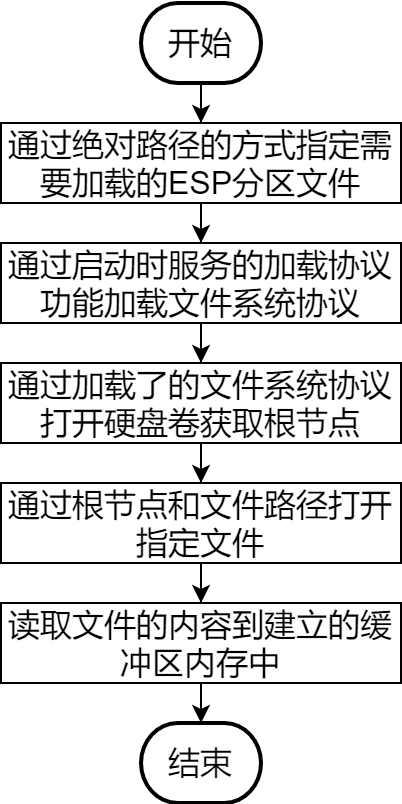
\includegraphics[width=4cm]{esp_file_load.png}
    % 中文标题 %
    \caption*{图 4-3 加载硬盘文件流程}
    % 调整图片英文标题与下文距离(本文标准为-0.7cm) %
    \setlength{\belowcaptionskip}{-0.7cm}
    % 英文标题 %
    \caption*{Figure 4-3 Process of loading hard disk files}
\end{figure}

首先需要通过Boot Service的HandleProtocol服务来加载系统提供的
EFI\_SIMPLE\_FILE\_SYSTEM\_PROTOCOL文件系统协议,将其安装在提供的Handle句柄上。然后调用协议中的OpenVolume
打开硬盘卷文件,将信息挂载到RootIo这个EFI\_FILE结构中,这个结构对应的是UEFI文件系统协议栈里的FileIo协议。
然后就是通过提供的具体文件相对路径,通过EFI\_FILE\_READ\_ONLY文件只读模式将其打开到FileIo,并通过文件协议
中的Read方法读取文件内容到指定地址。

\subsection{驱动文件度量模块}
驱动文件度量模块是此安全方案的核心内容,因为此模块需要负责对UEFI文件系统协议栈的四个驱动程序进行可信度量,
以确保他们的内容不被非法篡改。在有了固件文件系统访问模块的基础上,已经可以获取到FV固件中的驱动文件内容,
而度量模块,需要对加载到UEFI内存中的驱动文件内容进行信息匹配,以确保进行特定驱动程序的度量工作。因此需要
根据UEFI规范,确定四个驱动程序的GUID内容,以进行匹配。

\begin{lstlisting}
[Defines]
    BASE_NAME       = DiskIoDxe
    FILE_GUID       = 6B38F7B4-AD98-40e9-9093-ACA2B5A253C4
    ...
[Defines]
    BASE_NAME       = PartitionDxe
    FILE_GUID       = 1FA1F39E-FEFF-4aae-BD7B-38A070A3B609
    ...
[Defines]
    BASE_NAME       = AtaAtapiPassThruDxe
    FILE_GUID       = 5E523CB4-D397-4986-87BD-A6DD8B22F455
    ...
[Defines]
    BASE_NAME       = FatFileSys
    FILE_GUID       = a6a0274b-78da-4b77-8fb2-9c355a2e7f6a
    ...
\end{lstlisting}

如上面代码清单所示,四个UEFI文件系统协议栈驱动的GUID分别标注在了四个驱动INF模块文件的[Defines]字段中。
在确定了GUID后,就需要在度量功能的代码中进行GUID的匹配,再进行驱动数据内容的度量。需要说明的是,在四个
驱动程序中,由于UEFI使用的GPT分区格式和各个硬件设计为统一格式,因此PartitionDxe和DiskIoDxe驱动在各个
真机平台上是统一的;而PassThruDxe和FileSys驱动需要根据不同的物理平台确定不同的驱动和特定GUID。这里采用
的是申威6A型号服务器的具体驱动名称和GUID信息\cite{chinese7,addition2}。
\par 在驱动度量模块中,另一个重要的功能就是生成度量日志的功能。此功能的目的是向BMC系统发送UEFI启动过程
中度量UEFI文件系统协议栈的四个驱动和特定硬盘ESP分区文件时,将度量过程中产生的hash值和BMC中取出的基准值,
以及度量结果通过日志写入的方式,存储于BMC系统固件中。由于此功能不需要UEFI系统和BMC系统尽心数据互送,只
需要UEFI系统单向得将ASCII码信息写入BMC系统,因此通信方式没有采用IPMI协议,而是通过IO端口映射的方式,将
数据流写入目的地址。

\begin{figure}[htb]
    % 调整图片与上文的垂直距离 %
    \vspace{0cm}   
    % 调整图片图片与中文标题、中文标题与英文标题距离 %
    \setlength{\abovecaptionskip}{0.3cm}
    % 引用/fig/目录中的图片文件 %
	\centering
    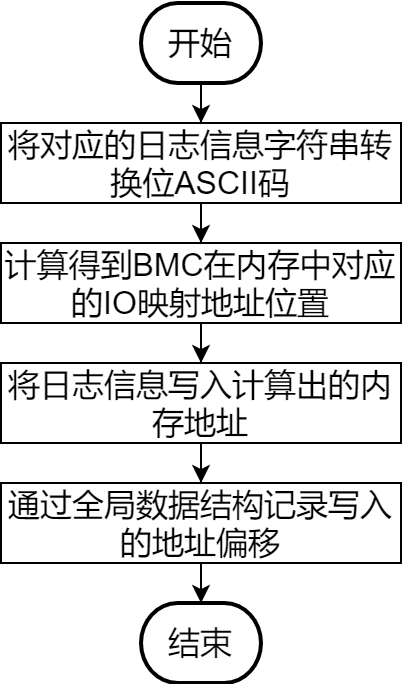
\includegraphics[width=4cm]{log_write.png}
    % 中文标题 %
    \caption*{图 4-4 日志信息写入流程}
    % 调整图片英文标题与下文距离(本文标准为-0.7cm) %
    \setlength{\belowcaptionskip}{-0.7cm}
    % 英文标题 %
    \caption*{Figure 4-4 Process of writing log information}
\end{figure}

如图4-4所示,描述的是度量日志写入功能中向串口写入信息的函数。其中输入的日志信息是使用系统调用AsciiVSPrint函数
后,通过DEBUG信息生成ASCII码格式的字符串。PRINTCONFIG结构用来在内存中表示打印信息参数的数据结构,用于记录每次Buffer需要写入的
目的地址,其中Start字段是PRINTCONFIG在内存中的起始地址,Index字段用于在每次写入以此Buffer数据后,自加一
以达到下次调用串口写入函数时,写入到上次数据内容的后面。IO映射地址的位置是
在系统DXE阶段初始化过程中确定的。值得注意的是,
这个串口写入函数是处理器体系结构相关的,因为PRINTCONFIG结构在计算地址时用到了cpuid值,并且在系统初始化时
PRINTK\_BUF\_CONFIG值的内容也是根据具体物理真机系统的自定义而决定的\cite{chinese13}。
\par 硬盘文件度量模块的逻辑与驱动度量模块相似,需要通过文件名来调用BMC通信模块,获取到BMC芯片中存储的文件
基准值信息,并在内存中通过SHA1算出加载前的度量值,进行比较得到度量结果。

\subsection{BMC通信模块}
BMC通信模块是图3-13中所示的,在此安全方案中,属于DXE阶段和BDS阶段所使用的与BMC系统通信的功能模块。由于
DXE和BDS阶段共同使用的是DXE阶段初始化的Boot Service和Runtime Service,因此保证了BMC通信模块中系统调用
的统一性。由于需要通过BMC通信模块获取基准值,因此不光需要向BMC发送数据,还需要BMC处理并返回对应的结果,
因此借助于IPMI协议来实现\cite{chinese26}。

\begin{lstlisting}
struct _EFI_IPMI_INTERFACE_PROTOCOL {
    EFI_IPMI_INTERFACE_SEND_COMMAND       SendCommand;
    EFI_IPMI_INTERFACE_RECEIVE_PACKET     ReceivePacket;
    EFI_IPMI_INTERFACE_GET_STATUS         GetStatus;
};
\end{lstlisting}
如上面的代码清单所描述,DXE阶段的BMC通信模块定义了一个名为EFI\_IPMI\_INTERFACE\_PROTOCOL的IPMI通信协议
结构体,其中包含了三个主要的函数指针。SendCommand函数用于通过UEFI系统向BMC系统发送IPMI格式的命令代码,
ReceivePacket函数用于在UEFI系统中读取BMC系统写入特定硬件缓存并通过UEFI的IO端口映射到内存中的地址,
GetStatus函数则用于读取特定的BMC寄存器,并按位解析BMC状态信息\cite{addition7}。
\par BMC通信模块以DxeInitlizeIpmiKcs作为入口函数,加载对应的IPMI协议中三个主要功能函数到Protocol数据
结构中,并通过gBS->InstallMultipleProtocolInterfaces,Boot Service中的安装协议函数通过
gEfiIpmiInterfaceProtocolGuid协议的全局标识信息,安装于EFI\_IPMI\_INSTANCE结构的Handle字段中。

\subsubsection{发送数据过程}
发送函数接收主要的8位标识的命令信息,和命令
数据大小,然后根据IPMI协议提供的KCS数据发送状态流,依次设置KCS命令和查询相关寄存器,配合数据接收寄存器的
数据写入过程\cite{english22}。代码的写入流程如图4-5。

\begin{figure}[htb]
    % 调整图片与上文的垂直距离 %
    \vspace{0cm}   
    % 调整图片图片与中文标题、中文标题与英文标题距离 %
    \setlength{\abovecaptionskip}{0.3cm}
    % 引用/fig/目录中的图片文件 %
	\centering
    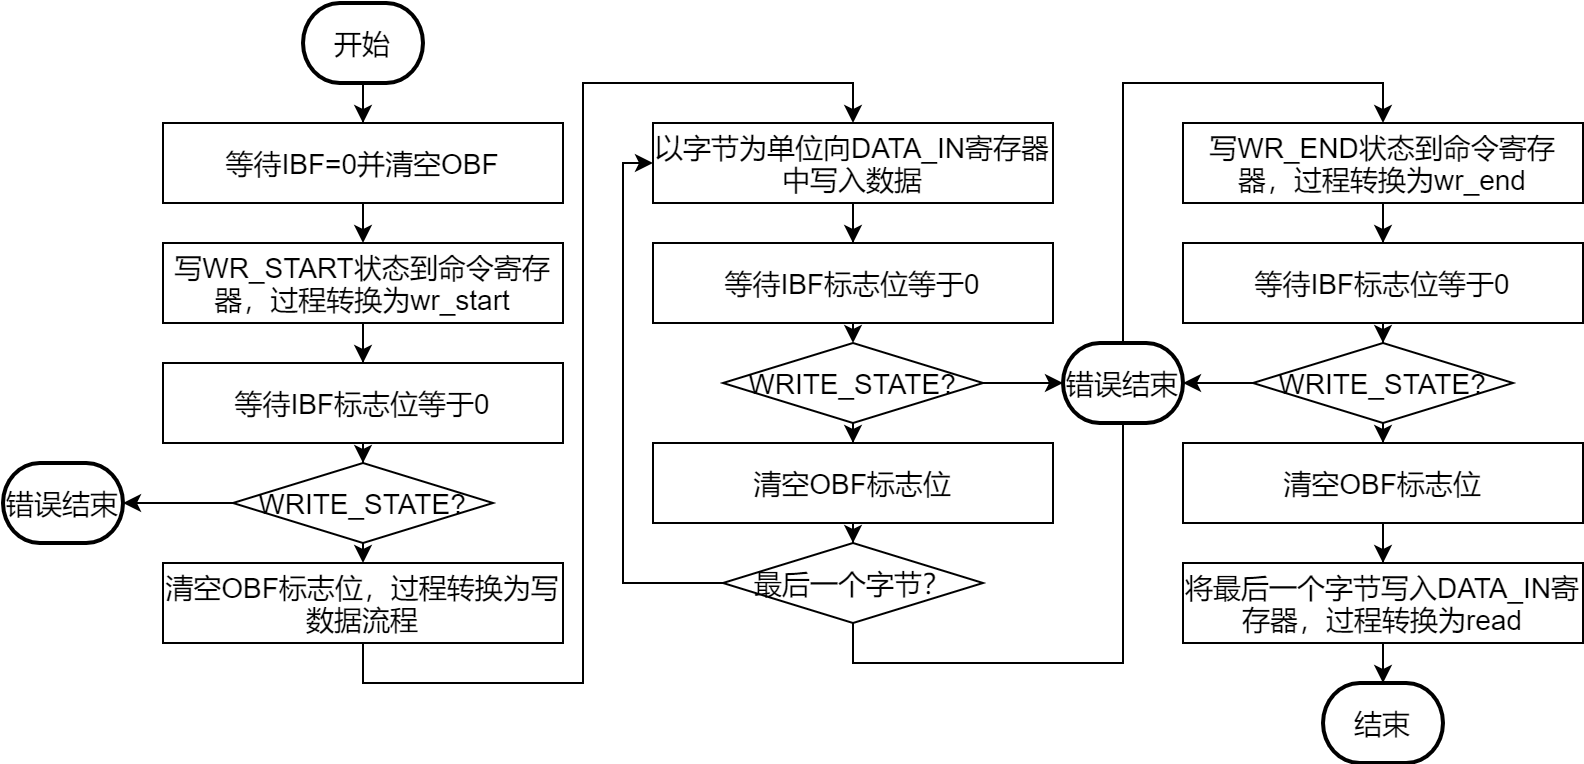
\includegraphics[width=14cm]{kcs_write_transfer.png}
    % 中文标题 %
    \caption*{图 4-5 kcs模式数据写入流程}
    % 调整图片英文标题与下文距离(本文标准为-0.7cm) %
    \setlength{\belowcaptionskip}{-0.7cm}
    % 英文标题 %
    \caption*{Figure 4-5 KCS Write Transfer Flow}
\end{figure}

如图4-5所示,是IPMI协议的KCS访问模式中数据写入BMC的执行流程,其中一共涉及到4种BMC寄存器的访问与操作,他们
包括Data\_In\_R、Data\_Out\_R、Status\_R和Command\_R,其中Status\_R是查询BMC状态的寄存器,Data\_Out\_R
和Data\_In\_R负责给BMC和外界系统如BIOS,提供数据的读出和写入缓存,用寄存器的方式来实现。Command\_R寄存器
用来表示输入BMC系统的命令。
\par 在图4-3中,首先等待Status\_R寄存器中的IBF标志位为0,表示此时没有数据输入到Data\_In\_R中。然后通过
将WRITE\_START命令写入Command\_R寄存器,将BMC状态改变为wr\_start写入开始状态。随后通过查询Status\_R中的值,
等待IBF标志位为0,表示BMC收到了WRITE\_START命令并判别有效;同时通过8位的状态寄存器获取到的值确认BMC此时的
状态确实改变为了WRITE\_STATE。后面就进入了数据写入的循环中,由于KCS模式是按字节传输数据,因此为Command\_R
寄存器设置两个命令分别为WRITE\_START和WRITE\_END来确定传入缓冲寄存器中的第一个和最后一个字节为单位的数据包。
每写入一个字节的数据之后,都要通过Status\_R检查IBF位,确定数据输入是否有效,同时检查BMC是否还保持WRITE\_STATE
状态。当根据数据size判断下一个字节是最后一个传输字节时,退出写入循环,并向Command\_R写入WRITE\_END命令,
来通知BMC下一个字节是最后一个。写入最后一个字节的流程和前面循环中的写入流程一致。最后BMC的状态转换成了read,
表示等待外部系统读取Data\_Out\_R中的返回值。

\begin{table}[htb]
    % 设置表内行间距 %
    \renewcommand\arraystretch{1.3}
    % 设置表题目 %
	\caption*{表 4-2 BMC状态寄存器标志位说明}
	\caption*{Table 4-2 KCS Interface Status Register Bits}
    \begin{tabular*}{\hsize}{@{\hspace{20pt}}@{\extracolsep{\fill}}ccl@{}}
    % 表上线和表头 %
	\toprule[0.75pt]
    比特位  &名称  &\makecell[c]{描述}\\
    % 表中线和表内容 %
    \midrule[0.5pt]
    0                             &OBF       &\quad 输出数据有效标志位\\
    1                             &IBF       &\quad 输入数据有效标志位\\
    2                             &SMS\_ATN  &\quad 表明BMC有事务需要软件系统处理\\
    3                             &C\_D\_n   &\makecell[l]{
                                              \quad 表明最后写入的是Command\_R还是\\
                                                    Data\_In\_R,“1”表示 Command\_R\\
                                            }\\
    5:4                          &OEM       &\quad 保留标志位\\
    7:6                          &S1:S0     &\quad KCS读写状态机状态\\
    % 表下线 %
	\bottomrule[0.75pt]
    \end{tabular*}
    % 表格与下文距离 %
    \vspace{-0.3cm}
\end{table}

如表4-2所示,其中7:6也就是bit7和bit6形成一个四种情况的状态组合,有限状态机组合情况如下:
\par 00:IDLE\_STATE,表示KCS接口是空闲的,外部系统不应预期收到或向其发送任何数据。
\par 01:READ\_STATE,读状态表示BMC正在向外部系统传输一个一字节大小的数据包,此时外部系统也应处于对应的
读取信息状态。
\par 10:WRITE\_STATE,写状态表示BMC正在从外部系统接收一个数据包,此时外部系统需要向BMC写入一个命令。
\par 11:ERROR\_STATE,表示BMC在接口级别检测到协议违规,或者传输已中止。外部系统可以使用Get\_Status
控制代码来请求错误的性质,也可以仅重新执行该命令。下面将介绍UEFI BIOS从BMC获取返回值的流程。

\subsubsection{接收数据过程}
KCS访问模式下外部系统读取BMC数据过程,所使用到的寄存器信息与发送过程一致。如图4-6所示,由于在外部系统写入
数据到BMC后,BMC状态机转换位等待读取的状态,因此首先检查IBF标志位保证上一次输入BMC的数据有效后,检查状态
是否为READ\_STATE,此状态为读取BMC数据的循环判断状态。当状态有效时,在OBF为1,保证输出有效的情况下,读取
DATA\_OUT中的一字节数据,随后再向DATA\_IN中写入READ,通过外部系统将BMC设置为READ\_STATE,然后进入读取循环。
直到读取完最后一个字节后,并由外部系统写READ指令后,BMC改变自身状态为IDLE\_STATE,以此来退出读取循环,并
写入输出缓存一个dummy字节。外部系统读取dummy字节后,完成整个读取操作。

\begin{figure}[H]
    % 调整图片与上文的垂直距离 %
    \vspace{0cm}   
    % 调整图片图片与中文标题、中文标题与英文标题距离 %
    \setlength{\abovecaptionskip}{0.3cm}
    % 引用/fig/目录中的图片文件 %
	\centering
    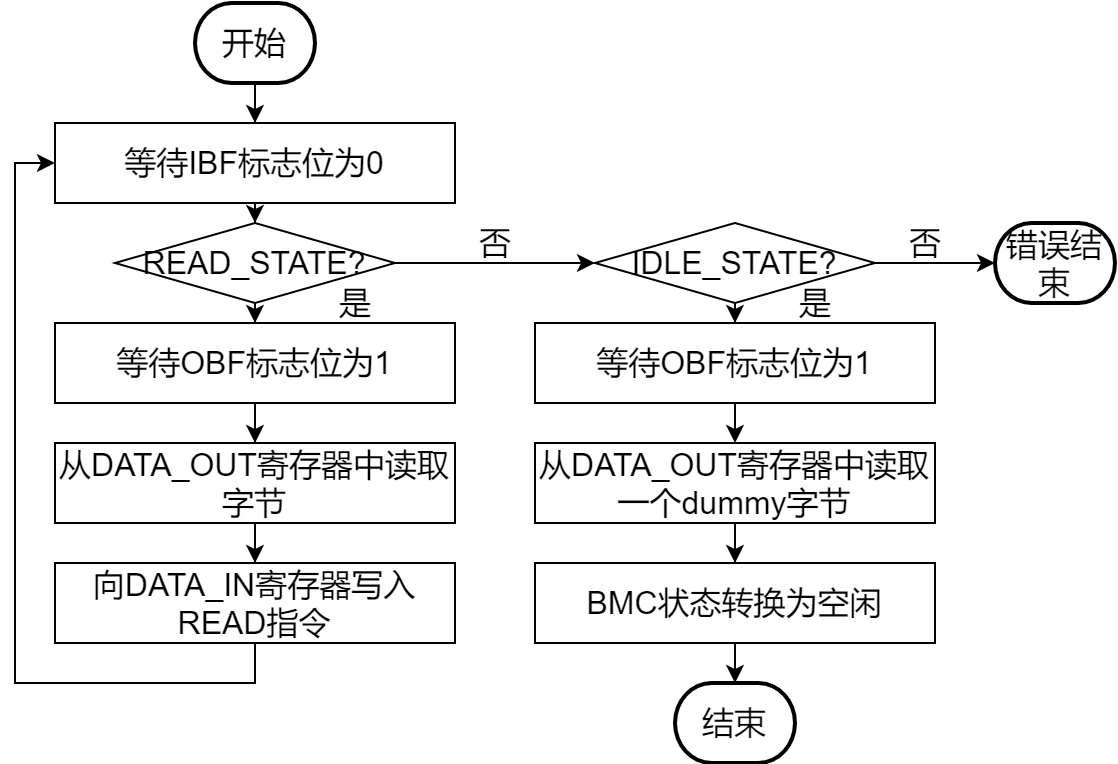
\includegraphics[width=10.6cm]{kcs_read_transfer.png}
    % 中文标题 %
    \caption*{图 4-6 kcs模式数据读取流程}
    % 调整图片英文标题与下文距离(本文标准为-0.7cm) %
    \setlength{\belowcaptionskip}{-0.7cm}
    % 英文标题 %
    \caption*{Figure 4-6 KCS Read Transfer Flow}
\end{figure}

%
% 4.2节
%
\section{UEFI启动阶段详细设计}

\subsection{SEC阶段设计}
由于SEC阶段是此可信链中的信任根,因此SEC阶段的数据内容安全可信,又因为SEC阶段占有很少的系统资源,仅有很小的
临时内存,因此不涉及BMC的交互功能,将SEC阶段度量PEI core的基准值信息,也就是PEI core的SHA1散列值,和临时的
SHA1算法,集成在SEC core的代码中,以此来完成阶段度量的任务。SEC阶段的BMC日志信息的输出由于不借助IPMI协议,
因此不需要BMC驱动程序,只需调用上述BMC串口写入函数,即可将日志信息写入BMC芯片中。

\begin{figure}[htb]
    % 调整图片与上文的垂直距离 %
    \vspace{0cm}   
    % 调整图片图片与中文标题、中文标题与英文标题距离 %
    \setlength{\abovecaptionskip}{0.3cm}
    % 引用/fig/目录中的图片文件 %
	\centering
    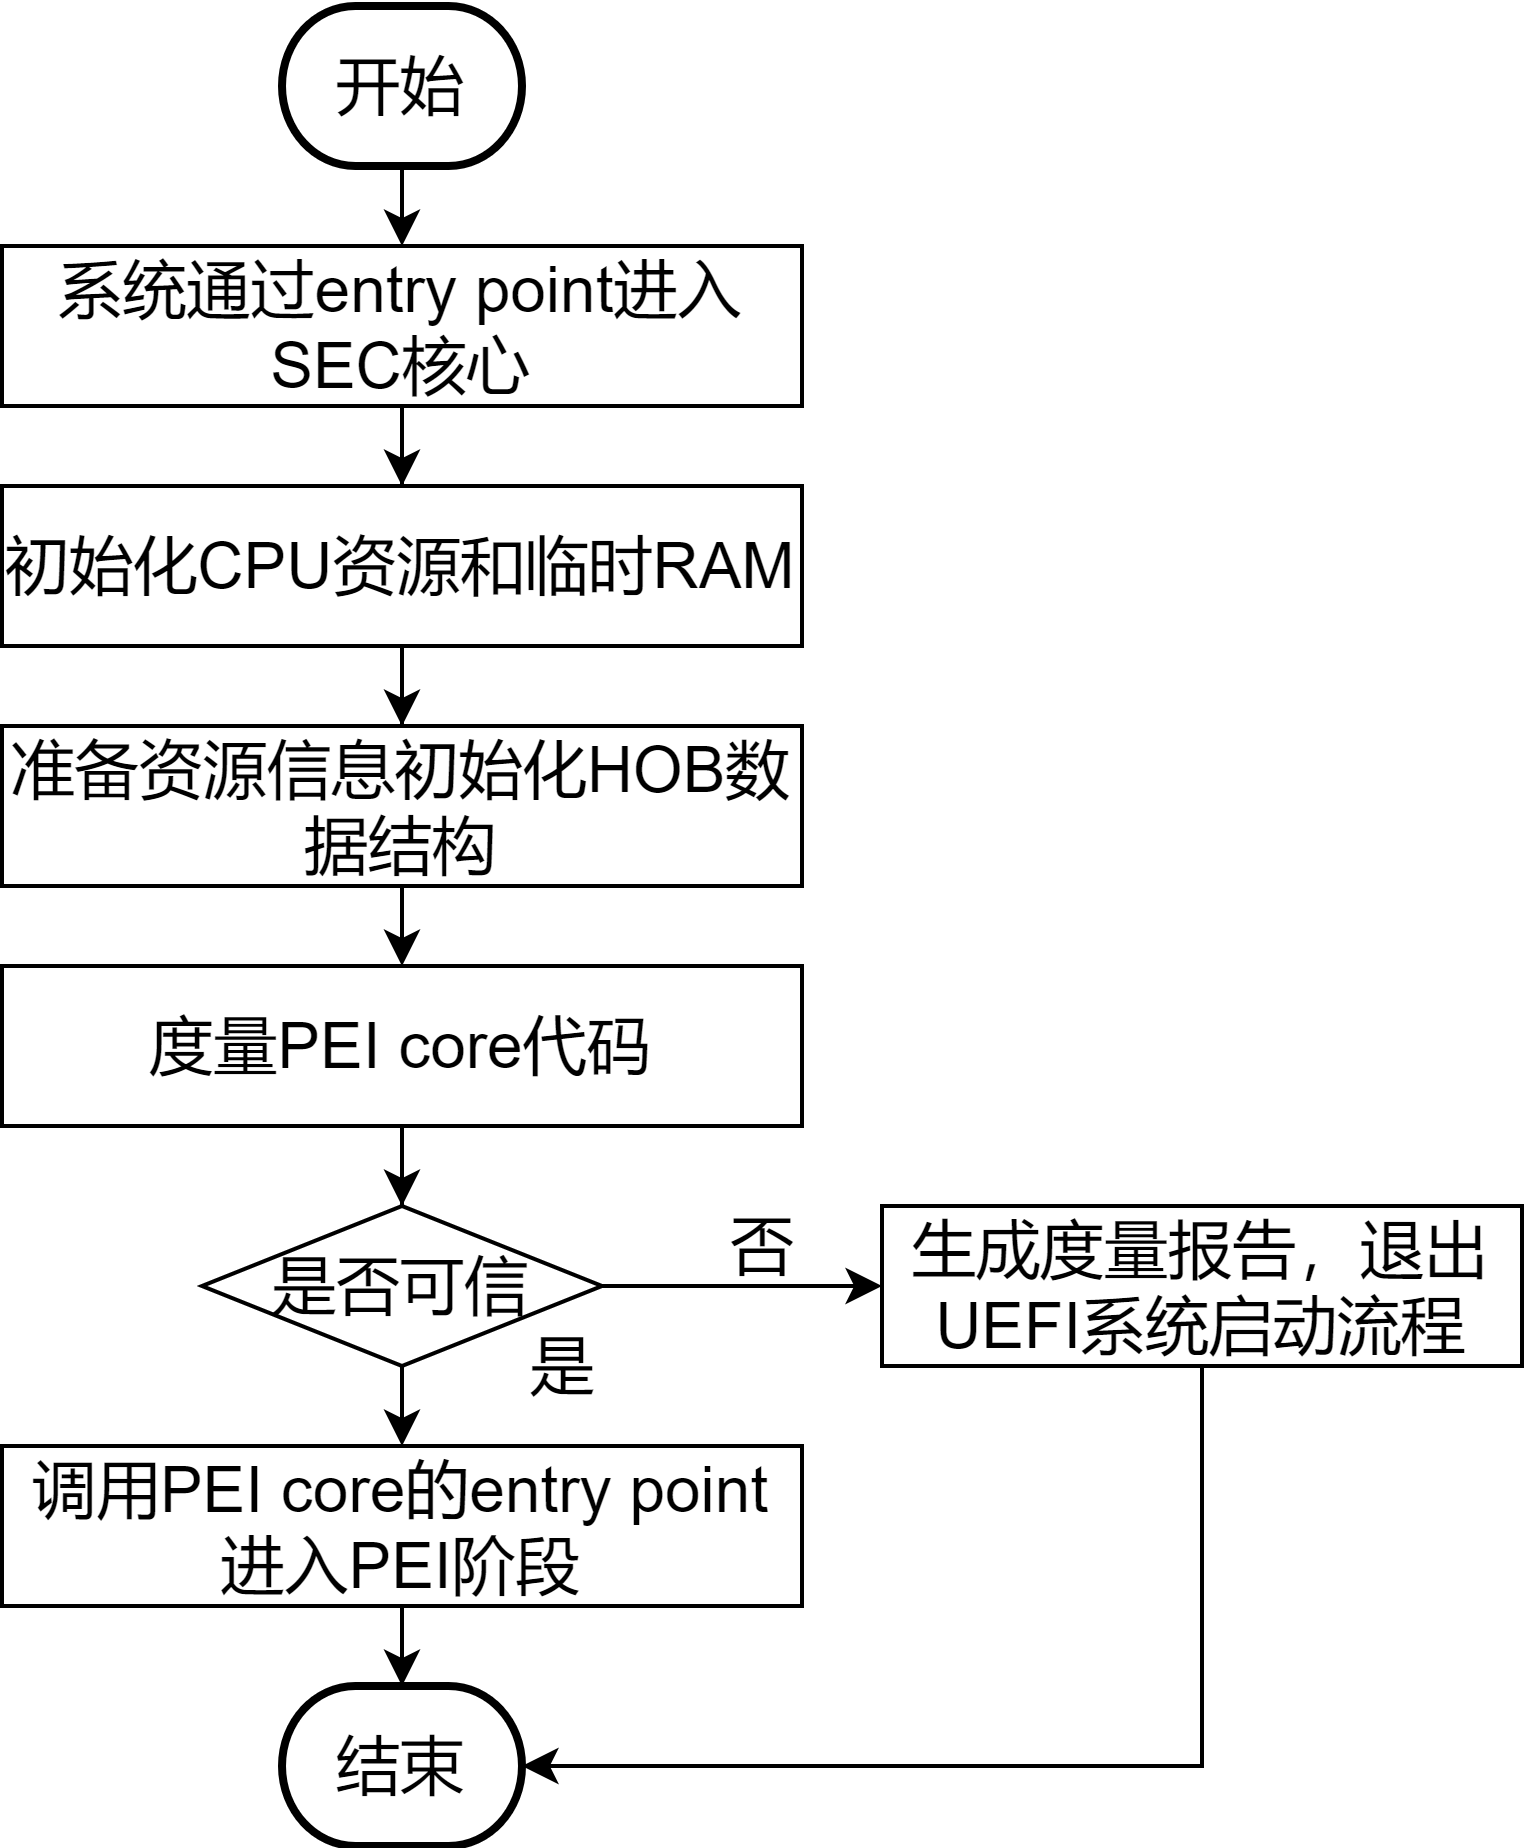
\includegraphics[width=8cm]{sec_process.png}
    % 中文标题 %
    \caption*{图 4-7 SEC阶段执行流程}
    % 调整图片英文标题与下文距离(本文标准为-0.7cm) %
    \setlength{\belowcaptionskip}{-0.7cm}
    % 英文标题 %
    \caption*{Figure 4-7 Execution process of SEC}
\end{figure}

如图4-7所示,在系统正常执行SEC阶段代码中加入可信度量PEI core代码的过程,并根据度量结果,若PEI core
内容可信,则控制权交给PEI的entry point入口函数,否则停止UEFI启动流程,并生成度量日志。

\subsection{PEI阶段设计}

\begin{figure}[htb]
    % 调整图片与上文的垂直距离 %
    \vspace{0cm}   
    % 调整图片图片与中文标题、中文标题与英文标题距离 %
    \setlength{\abovecaptionskip}{0.3cm}
    % 引用/fig/目录中的图片文件 %
	\centering
    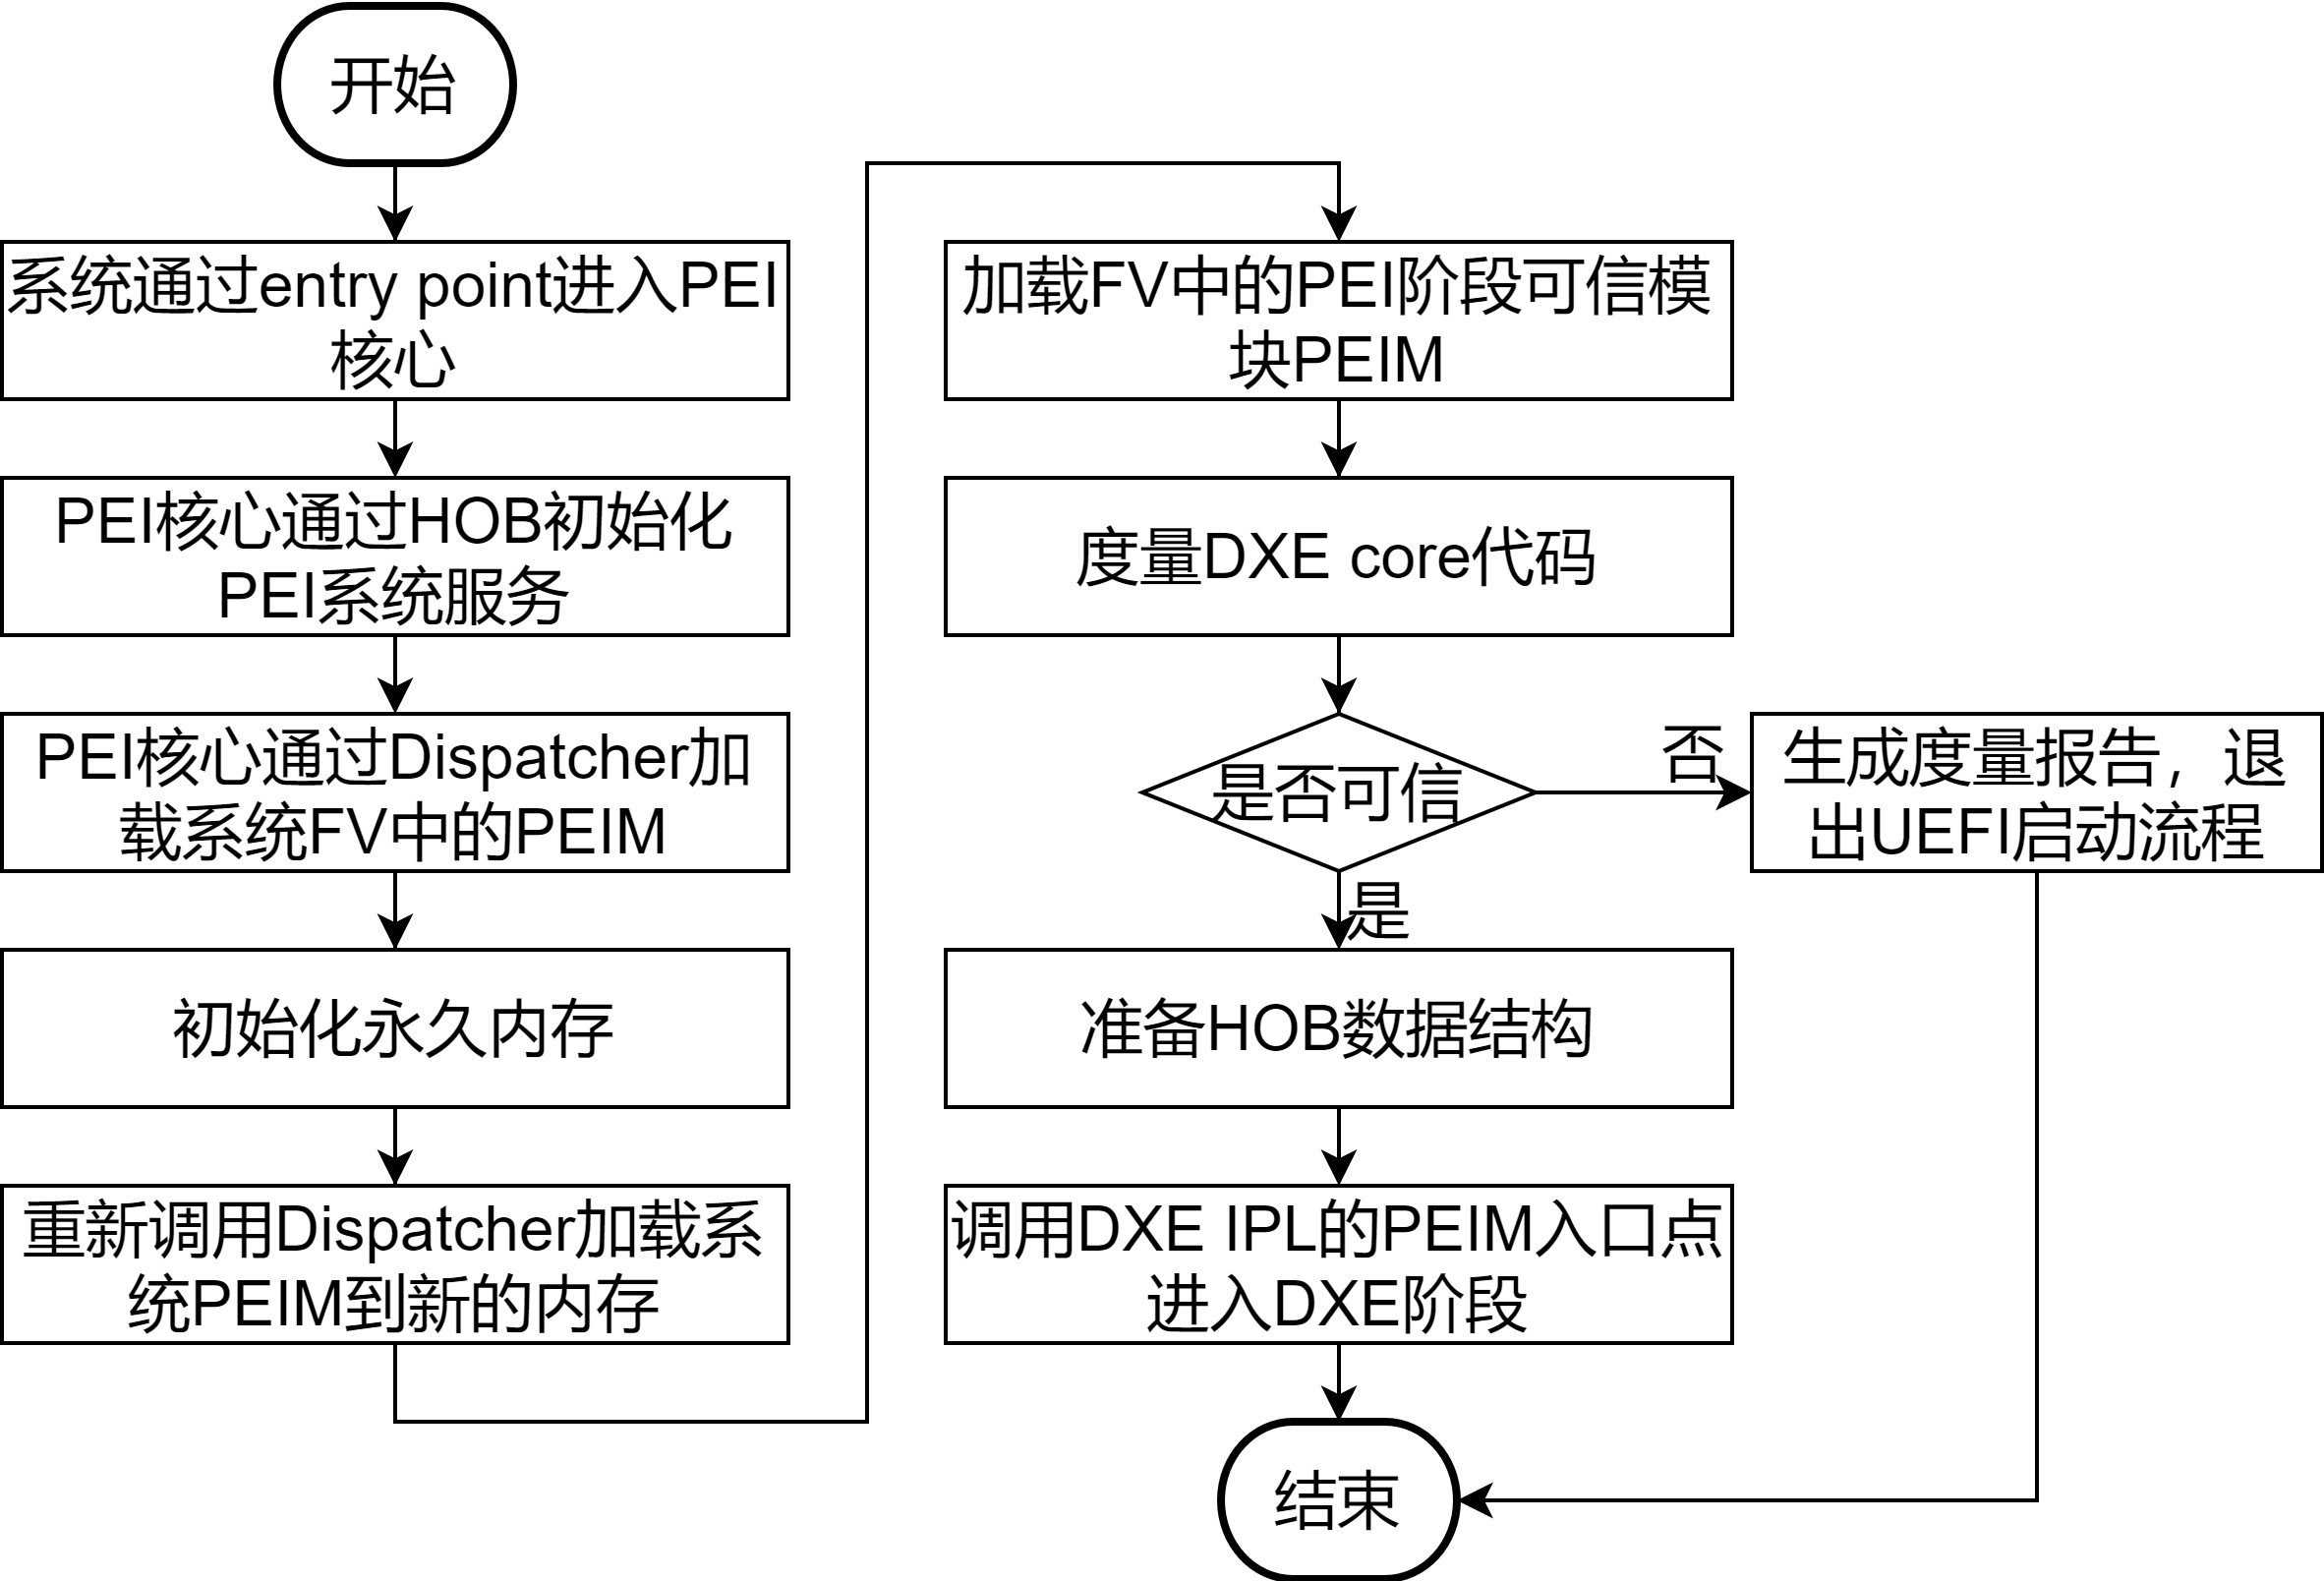
\includegraphics[width=12cm]{pei_process.png}
    % 中文标题 %
    \caption*{图 4-8 PEI阶段流程图}
    % 调整图片英文标题与下文距离(本文标准为-0.7cm) %
    \setlength{\belowcaptionskip}{-0.7cm}
    % 英文标题 %
    \caption*{Figure 4-8 Execution process of PEI}
\end{figure}

如图4-8所示,为本安全方案设计的PEI阶段流程。UEFI系统进入PEI阶段后,首先根据从SEC阶段传来
的HOB数据结构初始化PEI系统服务,用于给PEIM的加载过程提供支持;然后通过PEI阶段的调度程序加载
位于FV固件卷中的PEIM程序,除了cpu、主板和芯片组的PEIM外还包括如提供PPI通信协议的PEIM等内容;
随后PEI core通过这些最小的功能集合初始化UEFI系统的永久内存;在系统获得永久内存后,PEI core
再次调用PEIM调度程序,这次的目的是在完整的永久内存中加载这些PEIM,并在永久内存中执行后面流程;
随后加载FV中的PEI阶段的可信度量模块PEIM,用这个PEIM的功能度量FV中的DXE core代码,并根据度量
结果继续加载DXE core或是停止UEFI启动流程。

\par 由于PEI阶段设计为只度量DXE core核心代码,并且PEI阶段存在着两次驱动加载过程,分别是临时内存的关键PEIM
加载,这个目的是用最少的系统资源初始化post memory永久内存;永久内存建立后,再次调用PEIM的调度程序,将PEIM
加载到永久内存中。而DXE core入口函数需要在第二次永久内存中调用,因此,只需在第二次加载PEI阶段的可信度量PEIM
即可,这样可以减少系统不必要的加载PEIM带来的开销,具体流程如图3-10所示。
\par 在PEI阶段的PEIM调度程序中,会通过PEI core句柄中的FvPpi调用其中的GetFileInfo函数,将PEIM的信息存放在
EFI\_FV\_FILE\_INFO结构体中,因此可以通过EFI\_FV\_FILE\_INFO中的EFI\_GUID字段,来判断此PEIM是否为PEI
阶段的可信度量模块,若是,则通过EFI\_PEI\_SERVICES中的PeiMemoryInstalled布尔类型的变量来确定此次调度器
的调用是否在永久内存中,若是,再进行此可信度量模块的加载,否则跳过。由于PEI core和DXE core不是平台相关的,
因此大部分平台都会调用相同的EDKII实现的PEI和DXE核心程序和调度程序,此处提到的变量名称与EDKII开源项目中的名称
统一。

\subsection{DXE阶段设计}
DXE阶段为本安全方案度量UEFI文件系统协议栈驱动程序的主要系统启动阶段,目的是为后面BDS阶段通过
文件系统协议栈加载硬盘文件时,保证内核中文件系统服务程序的安全可靠。由于此安全方案的主要目的为
保证UEFI环境加载硬盘文件的安全可信,因此将DXE驱动度量范围缩小至UEFI文件系统协议栈相关驱动,
达到减小系统开销的目的。

\begin{figure}[htb]
    % 调整图片与上文的垂直距离 %
    \vspace{0cm}   
    % 调整图片图片与中文标题、中文标题与英文标题距离 %
    \setlength{\abovecaptionskip}{0.3cm}
    % 引用/fig/目录中的图片文件 %
	\centering
    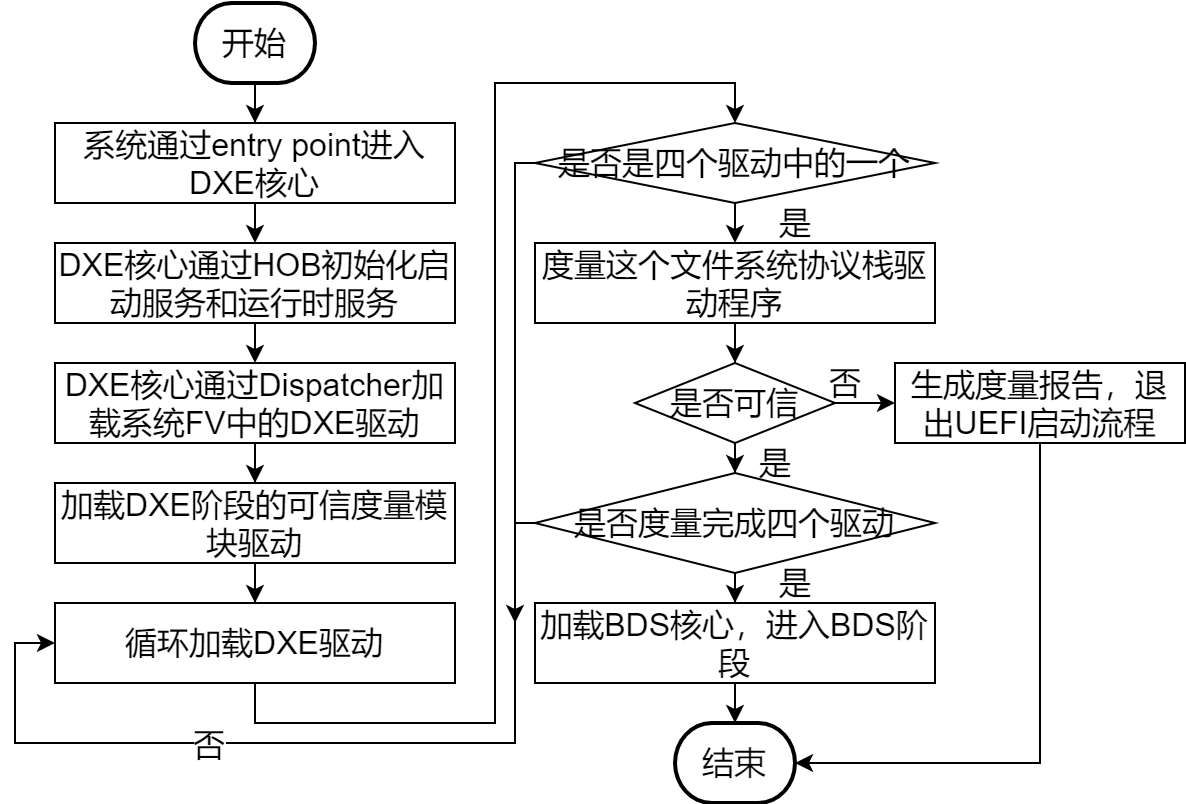
\includegraphics[width=12.3cm]{dxe_process.png}
    % 中文标题 %
    \caption*{图 4-9 DXE阶段流程图}
    % 调整图片英文标题与下文距离(本文标准为-0.7cm) %
    \setlength{\belowcaptionskip}{-0.7cm}
    % 英文标题 %
    \caption*{Figure 4-9 Execution process of DXE}
\end{figure}

如图4-9所示,系统进入DXE阶段后,首先根据PEI阶段传来的HOB数据结构初始化DXE阶段的Boot Service
和Runtime Service,用以给DXE阶段的驱动程序及其加载提供系统服务;随后控制权交给DXE阶段的调度
程序调度DXE驱动的加载,根据DXE驱动程序的依赖表达式,调度程序会首先加载那些系统相关度较低的驱动
程序,根据安全方案的设计,需要在加载UEFI文件系统协议栈的四个相关的驱动之前加载DXE阶段的可信度量
驱动。由于PEI和DXE两个阶段使用不同的系统服务,而可信度量模块中需要分别使用到PEI系统服务和DXE系统
服务,因此为PEI和DXE阶段分别设计两个可信度量功能的相关模块或驱动;之后在加载四个文件系统协议栈的
驱动程序前分别对其进行可信度量;根据四个驱动的可信度量结果,若都可信,则继续加载后续驱动并将系统
控制权最终交给BDS core,否则,停止UEFI系统启动。

\subsection{BDS阶段设计}
BDS core通过BDS架构协议定位和加载在启动准备服务环境中执行的各种各样的应用。这些应用可
能表示一个传统的OS启动装载程序,或者表示可代替最终的OS运行或在加载最终的OS之前运行的扩展服务。
这样的扩展启动准备服务可能包括安装配置、扩展诊断、闪存更新支持、OEM服务,或者OS启动代码。

\begin{figure}[htb]
    % 调整图片与上文的垂直距离 %
    \vspace{0cm}   
    % 调整图片图片与中文标题、中文标题与英文标题距离 %
    \setlength{\abovecaptionskip}{0.3cm}
    % 引用/fig/目录中的图片文件 %
	\centering
    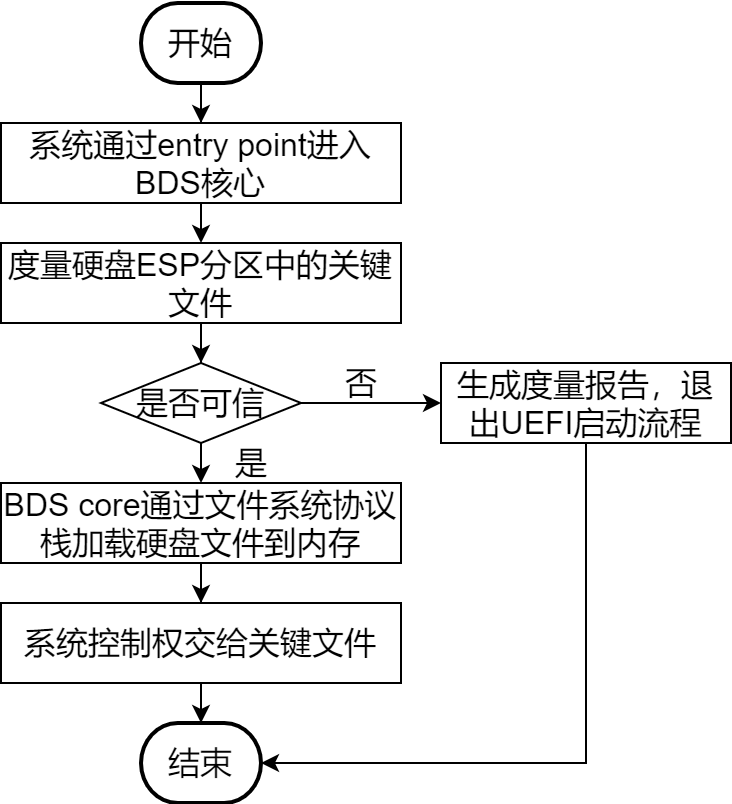
\includegraphics[width=8cm]{bds_process.png}
    % 中文标题 %
    \caption*{图 4-10 BDS阶段流程图}
    % 调整图片英文标题与下文距离(本文标准为-0.7cm) %
    \setlength{\belowcaptionskip}{-0.7cm}
    % 英文标题 %
    \caption*{Figure 4-10 Execution process of BDS}
\end{figure}

如图4-10所示,系统进入BDS阶段执行BDS core代码,并根据BDS加载的硬盘ESP分区中的文件调用DXE阶段
加载的可信度量服务型驱动对该文件进行可信度量,若结果可信,则通过UEFI文件系统协议栈加载此文件
到UEFI系统的永久内存中,并交给此文件系统的控制权;否则停止该文件的加载,退出UEFI启动。


\subsection{DXE阶段驱动依赖关系}
依赖关系是UEFI中一个调度程序相关的事项,存在于PEI调度程序和DXE调度程序中。由于PEI阶段的安全方案设计是通过
手动控制修改调度程序代码,来实现最后加载可信度量的PEIM,因此不存在依赖关系的建立。而DXE阶段驱动众多,需要
度量的文件系统协议栈驱动程序和BDS core代码项目也较多,因此需要借助UEFI提供的依赖关系表达式来实现可信度量
模块驱动在四个文件系统驱动前进行加载,这样才能在加载四个文件系统驱动时调用可信度量驱动中的IPMI协议来实现
系统加载驱动前进行度量。
\par 依赖关系表达式存储于图4-1中对应的dependency section中,存储在依赖项部分中的依赖项表达式设计得较小,
以节省空间。另外,它们的设计理念为简单、快速,以减少执行开销。通过设计一个小的基于堆栈的指令集来对依赖项
表达式进行编码,可以实现这两个目标。DXE分派器必须为此指令集实现一个解释器,以便评估依赖项表达式。

\begin{table}[H]
    % 设置表内行间距 %
    \renewcommand\arraystretch{1.3}
    % 设置表题目 %
	\caption*{表 4-3 依赖表达式命令摘要}
	\caption*{Table 4-3 Dependency Expression Opcode Summary}
    % @{\hspace{0pt}}用来表示表中每列的间隔 %
    \begin{tabular*}{\hsize}{@{\hspace{0pt}}ccl@{\hspace{0pt}}}
    % 表上线和表头 %
	\toprule[0.75pt]
    执行代码  &命令  &\makecell[c]{描述}\\
    % 表中线和表内容 %
	\midrule[0.5pt]
    0x00    &BEFORE <File Name GUID>  &\quad 在提供的GUID表示的驱动前加载此驱动\\
    0x01    &AFTER <File Name GUID>   &\quad 在提供的GUID表示的驱动后加载此驱动\\
    0x02    &PUSH <Protocol GUID>     &\makecell[l]{
                                       \quad 向栈中添加一个布尔类型的变量,如果这\\
                                             个GUID表示的协议在句柄数据库中,则添\\
                                             加TRUE,否则添加FALSE\\
                                        }\\
    0x03    &AND                      &\quad 与运算,用于判断栈中判断结果\\
    0x04    &OR                       &\quad 或运算,用于判断栈中判断结果\\
    0x05    &NOT                      &\makecell[l]{
                                       \quad 出栈一个布尔值,通过非运算计算后,将\\
                                             结果添加进栈\\
                                        }\\
    0x06    &TRUE                     &\quad 表示总判断结果为真\\
    0x07    &FALSE                    &\quad 表示总判断结果为假\\
    0x08    &END                      &\quad 依赖表达式的结束标志符\\
    0x09    &SOR                      &\quad 表示驱动还未加载,等同于NOP效果\\
    % 表下线 %
	\bottomrule[0.75pt]
    \end{tabular*}
    % 表格与下文距离 %
    \vspace{-0.3cm}
\end{table}

如表4-3所示,是DXE阶段的依赖表达式命令集,PEI阶段的依赖表达式除了没有BEFORE和AFTER之外,其他命令与
DXE阶段相同。UEFI系统中,通过INF文件的[Protocols]字段下添加协议名称,可以通过EDKII的BaseTool目录下
的依赖表达式相关的词法语法分析器,形成对应的依赖表达式,并通过编译存储与驱动文件的dependency section中。
除了通过这种方式,还可以通过手写依赖文件的方式确定驱动的加载优先级。通过编写后缀名为dxs的驱动依赖文件,
也可以达到将此信息写入FV中驱动的dependency section的目的。
\par 在DXE调度器解析dependency section时,会根据每一个GUID向依赖栈中压入句柄数据库中此协议或驱动的
查询结果,然后发现END结束符时,在通过AND这样的各个结果判断关系,依次将布尔值出栈,最后通过最终的依赖
表达式确定此驱动是否在此轮进行调度加载。FV固件卷中的依赖表达式事例如图4-11。

\begin{figure}[htb]
    % 调整图片与上文的垂直距离 %
    \vspace{0cm}   
    % 调整图片图片与中文标题、中文标题与英文标题距离 %
    \setlength{\abovecaptionskip}{0.3cm}
    % 引用/fig/目录中的图片文件 %
	\centering
    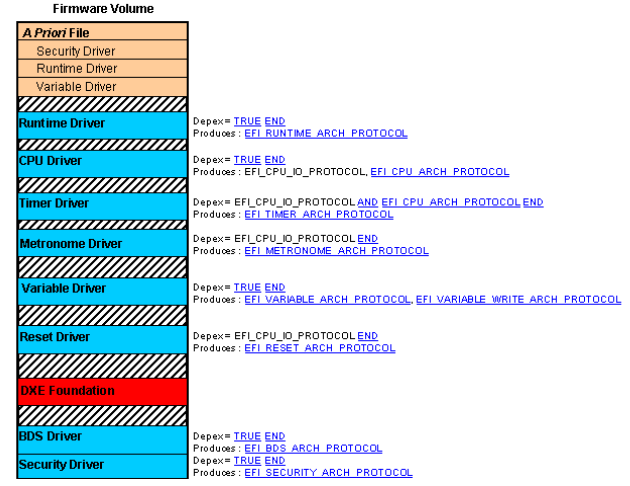
\includegraphics[width=10cm]{fv_depex.png}
    % 中文标题 %
    \caption*{图 4-11 固件卷依赖表达式存储}
    % 调整图片英文标题与下文距离(本文标准为-0.7cm) %
    \setlength{\belowcaptionskip}{-0.7cm}
    % 英文标题 %
    \caption*{Figure 4-11 Dependency Expression In Firmware Volume}
\end{figure}

如图4-11所示,FV中有一个Priori File用来描述系统规定的强类型优先级关系,即这个优先级文件中规定的加载顺序
必须严格按照规定执行。而依赖表达式则属于弱类型优先关系,原因是UEFI通过一个队列来控制每一轮通过调度程序
加载驱动,依赖表达式只能保证若此轮此驱动所依赖的协议或其他驱动已加载完成,则保证此驱动在此轮加载,而不能
保证的是此驱动的精确加载顺序。如图中所示,Security、Runtime和Variable驱动严格按照顺序加载,而依赖于CPUIO
协议的Metronome和Reset驱动则只要系统完成CPUIO协议的加载,则加载这两个驱动,但不能保证这两个驱动加载的
先后顺序,因此名为弱类型。
\par 此安全方案中驱动顺序的具体调整,就是通过在四个文件系统协议栈驱动程序的INF文件中的[Depex]字段下
添加可信度量驱动所生成的IPMI协议和SHA1计算协议即可。也可通过编写dxs依赖文件来对可信度量驱动和四个文件系统
协议栈驱动程序的加载顺序进行自定义,实现方法如下。

\begin{lstlisting}
DEPENDENCY_START
    EFI_SHA1_PROTOCOL_GUID                    AND
    EFI_IPMI_INTERFACE_PROTOCOL_GUID
DEPENDENCY_END
\end{lstlisting}
\par 最后在四个UEFI文件系统协议栈驱动程序的INF文件的[nmake.common]字段下,引用依赖文件DPX\_SOURCE=
FileSysStack.dxs,从而将dxs文件添加进驱动文件的编译过程。

%
% 4.3节
%
\section{本章小结}
本章节介绍了此安全方案的各个模块的详细设计即关键数据结构和协议的代码实现,其主要包括DXE和BDS阶段
起作用的可信度量驱动,也包括其中的驱动文件度量模块、硬盘文件度量模块、hash算法模块和BMC通信模块,也有
负责缓存硬盘文件和FV中驱动文件的中间层模块。然后介绍了PEI和DXE阶段分成两个可信度量驱动实现的理由,
以及SEC阶段、PEI阶段的详细设计思路,最后是DXE阶段依赖表达式的利用方法,以确保安全方案的实施。

\bjutclearpage
